\documentclass[17pt, t, lualatex]{beamer}



\title{Actividades, Grupos, Colectivos y Semilleros\footnote{Para sacar el máximo provecho a la matrícula :D } }
\date{\today}
\institute[UJTL]{Universidad Jorge Tadeo Lozano}
\author{Ludwig Alvarado Becerra}

\usepackage{amsmath, amssymb, mathtools}
\usepackage{graphicx}
\usepackage[spanish]{babel}
\usepackage{biblatex}
\usepackage{hyperref}
\usepackage{xurl}
\usepackage{svg}
\usepackage{listings}
\usepackage[scale=7]{ccicons}



\addbibresource{sample.bib}


\definecolor{white}{HTML}{FFFFFF}
\definecolor{sand}{HTML}{EBE5E0}
\definecolor{KTHblue}{HTML}{004791}
\definecolor{skyblue}{HTML}{6298D2}
\definecolor{navy}{HTML}{000061}
\definecolor{lightblue}{HTML}{DEF0FF}
\definecolor{digitalblue}{HTML}{0029ED}


\lstset{
  language=bash,                       % Set the language to bash
  backgroundcolor=\color{white},       % Background color for the code block
  basicstyle=\ttfamily\normalsize,    % Use typewriter font and small size
  keywordstyle=\color{KTHblue},           % Style for keywords (e.g. if, for, etc.)
  commentstyle=\color{sand},          % Style for comments
  stringstyle=\color{skyblue},             % Style for strings
  showstringspaces=false,              % Don't underline spaces in strings
  breaklines=true,                     % Automatically break long lines
  frame=single,                        % Add a frame around the code
  captionpos=b,                        % Position of the caption (bottom)
  numbers=left,                        % Line numbers on the left
  numberstyle=\tiny\color{gray},       % Style for line numbers
  stepnumber=1,                        % Display every line number
  numbersep=5pt,                       % Space between line numbers and code
  morekeywords={bat, wc, tail, cut, head, >},
}



% Probably load as late as possible
% Other options are
% - engine=pdflatex to compile in pdfLaTeX (with different fonts),
% - mathshape=rm to use serif font for math,
% - mathsahpe=custom to not set any math font (so that you can define your own math fonts)
\usetheme[engine=lualatex, mathshape=sf, fontdir=kthpq-files/fonts/Figtree/]{kthpq}
\setmonofont{Bitstream Vera Sans Mono}[Scale=.9]

% Custom colors (see beamercolorthemecustom.sty for more details)
% \usecolortheme{custom}

% Modify the headline template: KTH-full, KTH-section-only, or KTH-frametitle-only.
% \setbeamertemplate{headline}[KTH-full]

% Custom footline
% \setfootline{left}{center}{right}



\begin{document}

\inserttitlepage

\section{Índice}

\insertsectionpage

\begin{frame}
  \frametitle{Índice}
  \tableofcontents[hideallsubsections]
\end{frame}

\AtBeginSection[]{
  \begin{frame}
    \frametitle{Índice}
    \tableofcontents[currentsection, hideothersubsections]
  \end{frame}
}

\section{Deportes}

\begin{frame}
  \frametitle{Deportes}
  \begin{figure}
    \centering
    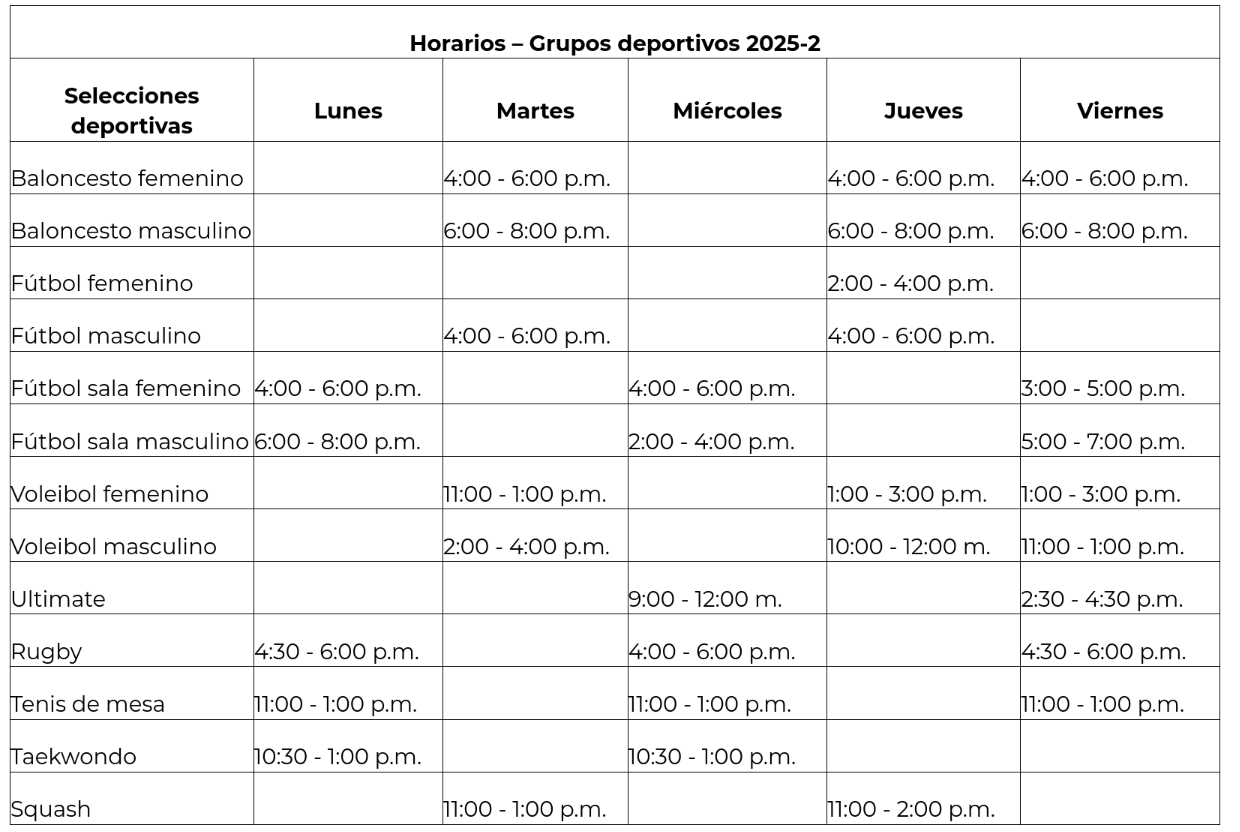
\includegraphics[height=0.9\textheight]{img/Deportes.png}
  \end{figure}

\end{frame}

\begin{frame}
  \frametitle{Deportes}
  \begin{columns}
    \begin{column}{.5\textwidth}
      \begin{itemize}
        \item Variedad de deportes.
        \item Estudiantes de todos los semestres y de todas las carreras.
        \item Más información en: \url{https://www.utadeo.edu.co/es/micrositio/deportes}
      \end{itemize}
    \end{column}

    \begin{column}{.5\textwidth}
      \begin{figure}
        \centering
        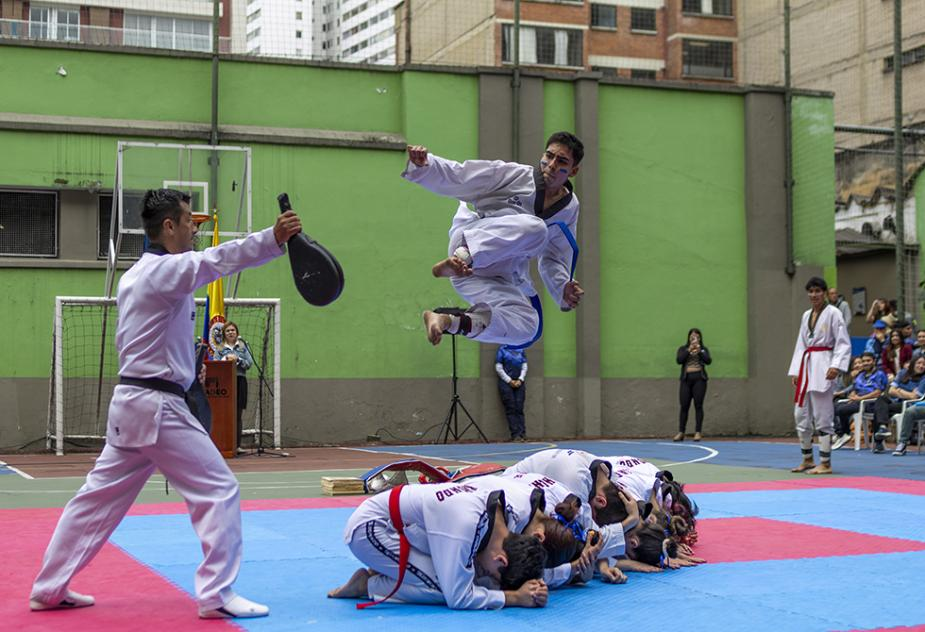
\includegraphics[width=0.8\textwidth]{img/TadeoOlimpiadas.jpg}
        \caption{Inauguración de las TadeOlimpiadas\cite{deportes2024}}
      \end{figure}
    \end{column}
  \end{columns}

\end{frame}


\section{Colectivo de Software Libre, GNUTADEO}

\insertsectionpage



\begin{frame}
  \frametitle{Colectivo de Software Libre, GNUTADEO}
  \begin{figure}
    \centering
    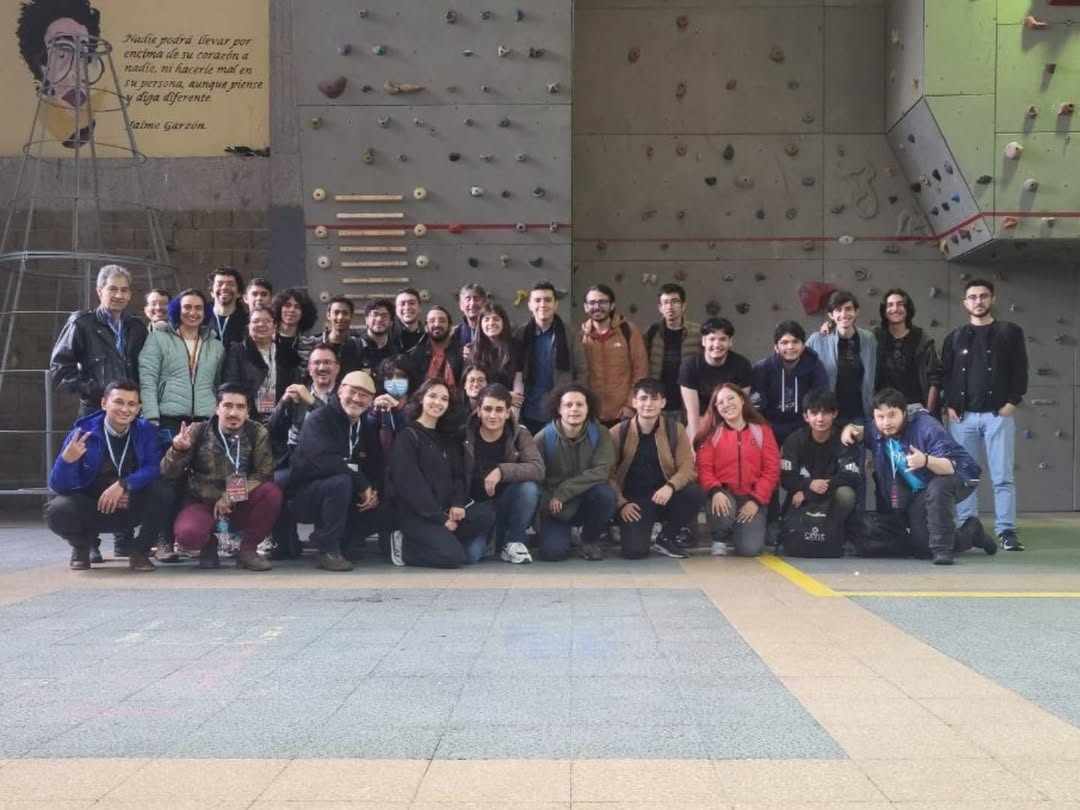
\includegraphics[height=0.85\textheight]{img/FLISOL2025.jpg}
    \caption{Participación FLISoL 2025}
  \end{figure}
\end{frame}

\begin{frame}
  \frametitle{Colectivo de Software Libre, GNUTADEO}
  \begin{figure}
    \centering
    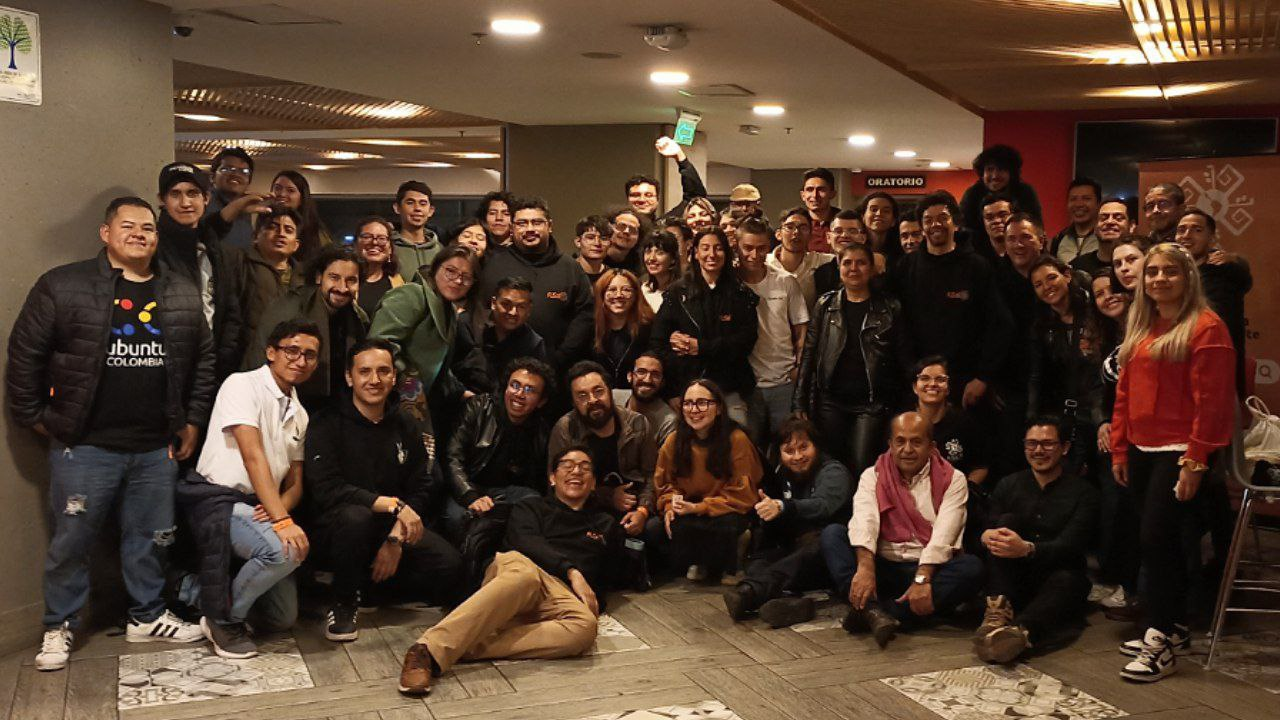
\includegraphics[height=0.85\textheight]{img/FLISOL2024.jpg}
    \caption{Participación FLISoL 2024}
  \end{figure}
\end{frame}




\section{Referencias}
\begin{frame}
  \frametitle{Referencias}
  \printbibliography

\end{frame}

\insertendpage

\end{document}
